\chapter{Конструкторская часть}

В данном разделе будут представлены схемы реализаций алгоритмов конвейерных вычислений, токенизации, применения правил к токенам и сортировки токенов по алфавиту. Также будет приведена общая схема алгоритма функции-обработчика для конвейерных вычислений.

\section{Разработка алгоритмов конвейерных вычислений}
На рисунке \ref{img:pipe} представлена схема реализации алгоритма линейных конвейерных вычислений и схема реализации алгоритма параллельных конвейерных вычислений, общая схема реализации функции-обработчика представлена на рисунке \ref{img:goroutine}. 

\begin{figure}[h!]
    \centering
    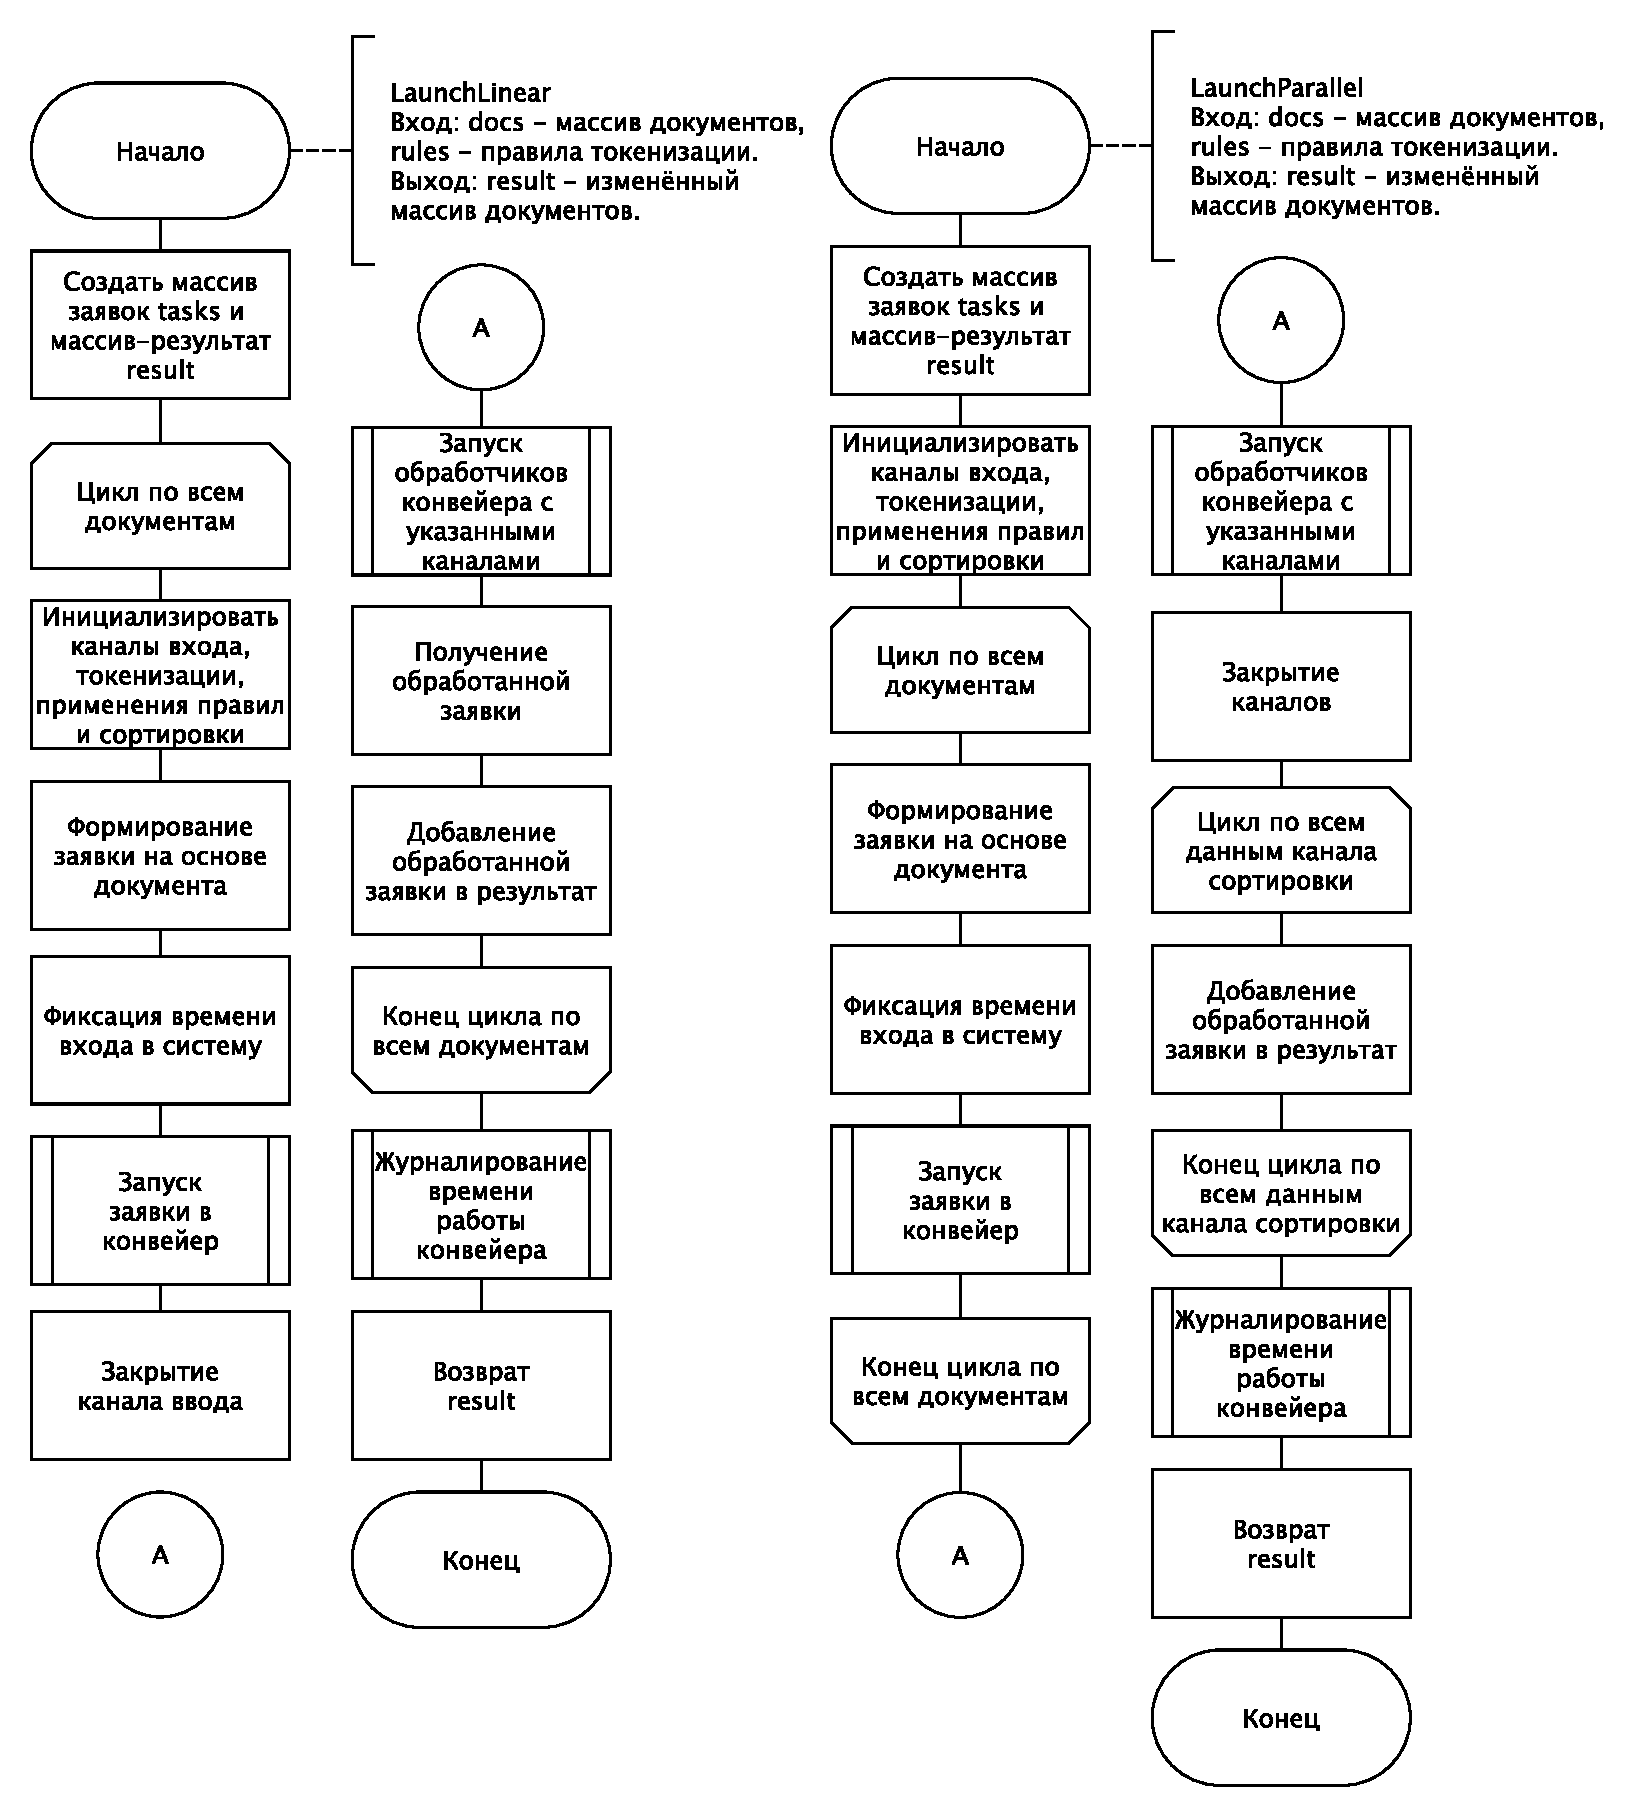
\includegraphics[width=0.7\linewidth]{pipe.pdf}
    \caption{Схема реализации алгоритма линейных конвейерных вычислений}
    \label{img:pipe}
\end{figure}

\begin{figure}[h!]
    \centering
    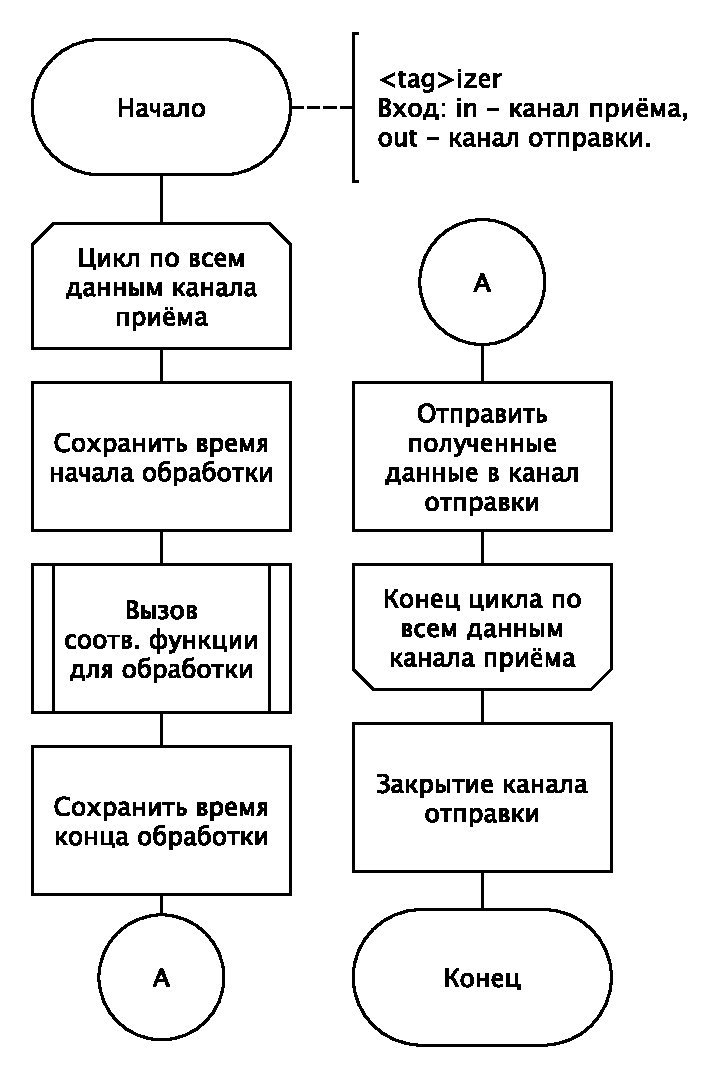
\includegraphics[width=0.35\linewidth]{goroutine.pdf}
    \caption{Общая схема реализации функции-обработчика для конвейерных вычислений}
    \label{img:goroutine}
\end{figure}

\section{Разработка алгоритма токенизации текста}
На рисунке \ref{img:token} представлена схема реализации алгоритма токенизации текста.

\begin{figure}[h!]
    \centering
    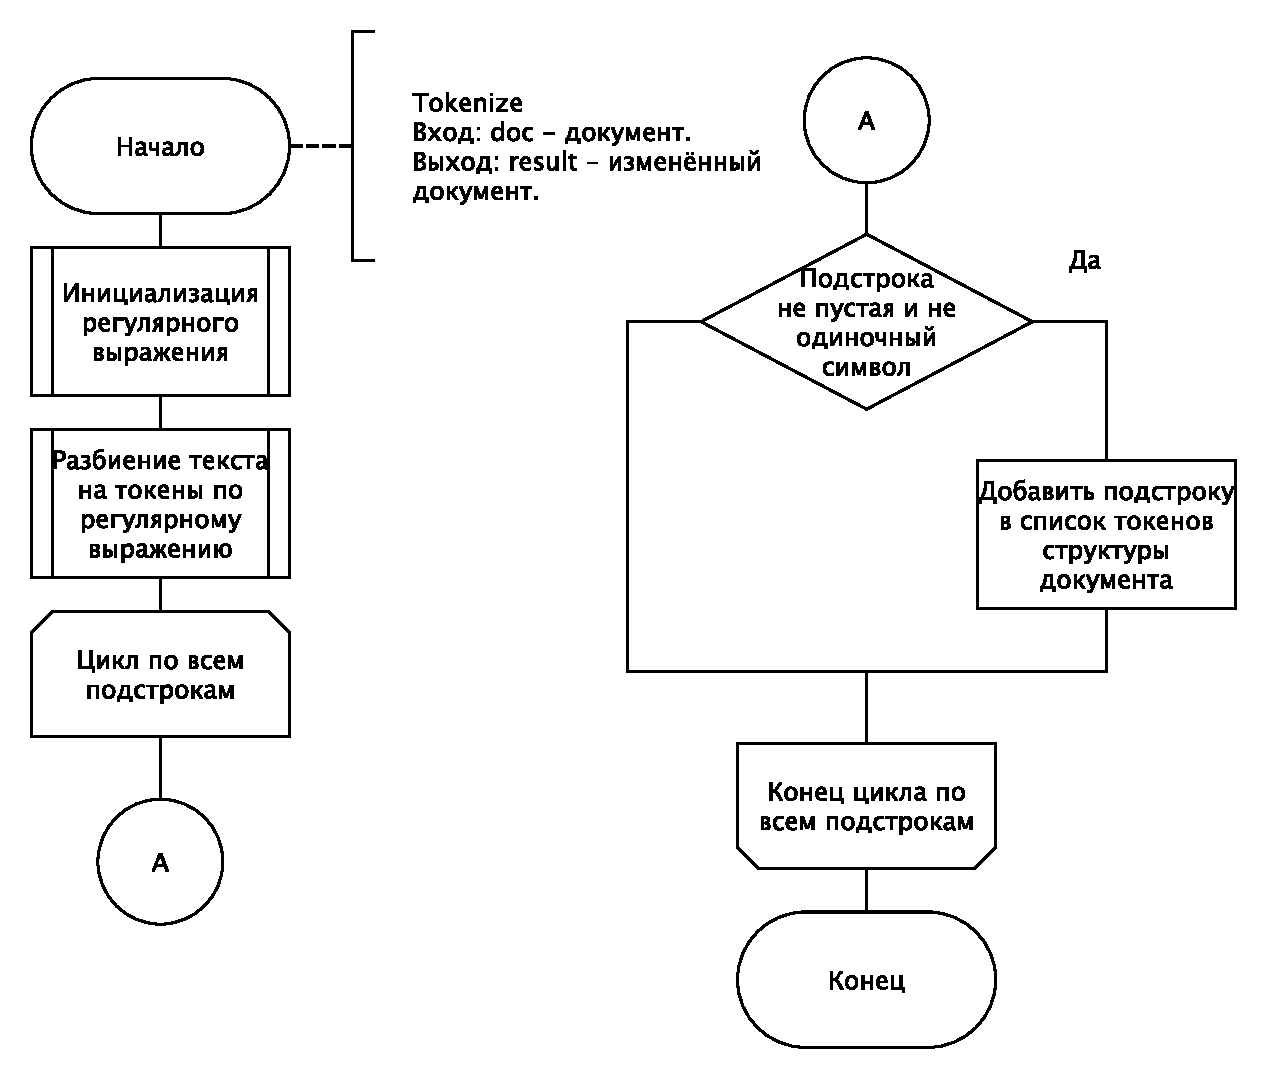
\includegraphics[width=0.54\linewidth]{token.pdf}
    \caption{Схема реализации алгоритма токенизации текста}
    \label{img:token}
\end{figure}

\section{Разработка алгоритма применения правил к токенам текста}
На рисунке \ref{img:rule} представлена схема реализации алгоритма применения правил к токенам текста. 

\begin{figure}[h!]
    \centering
    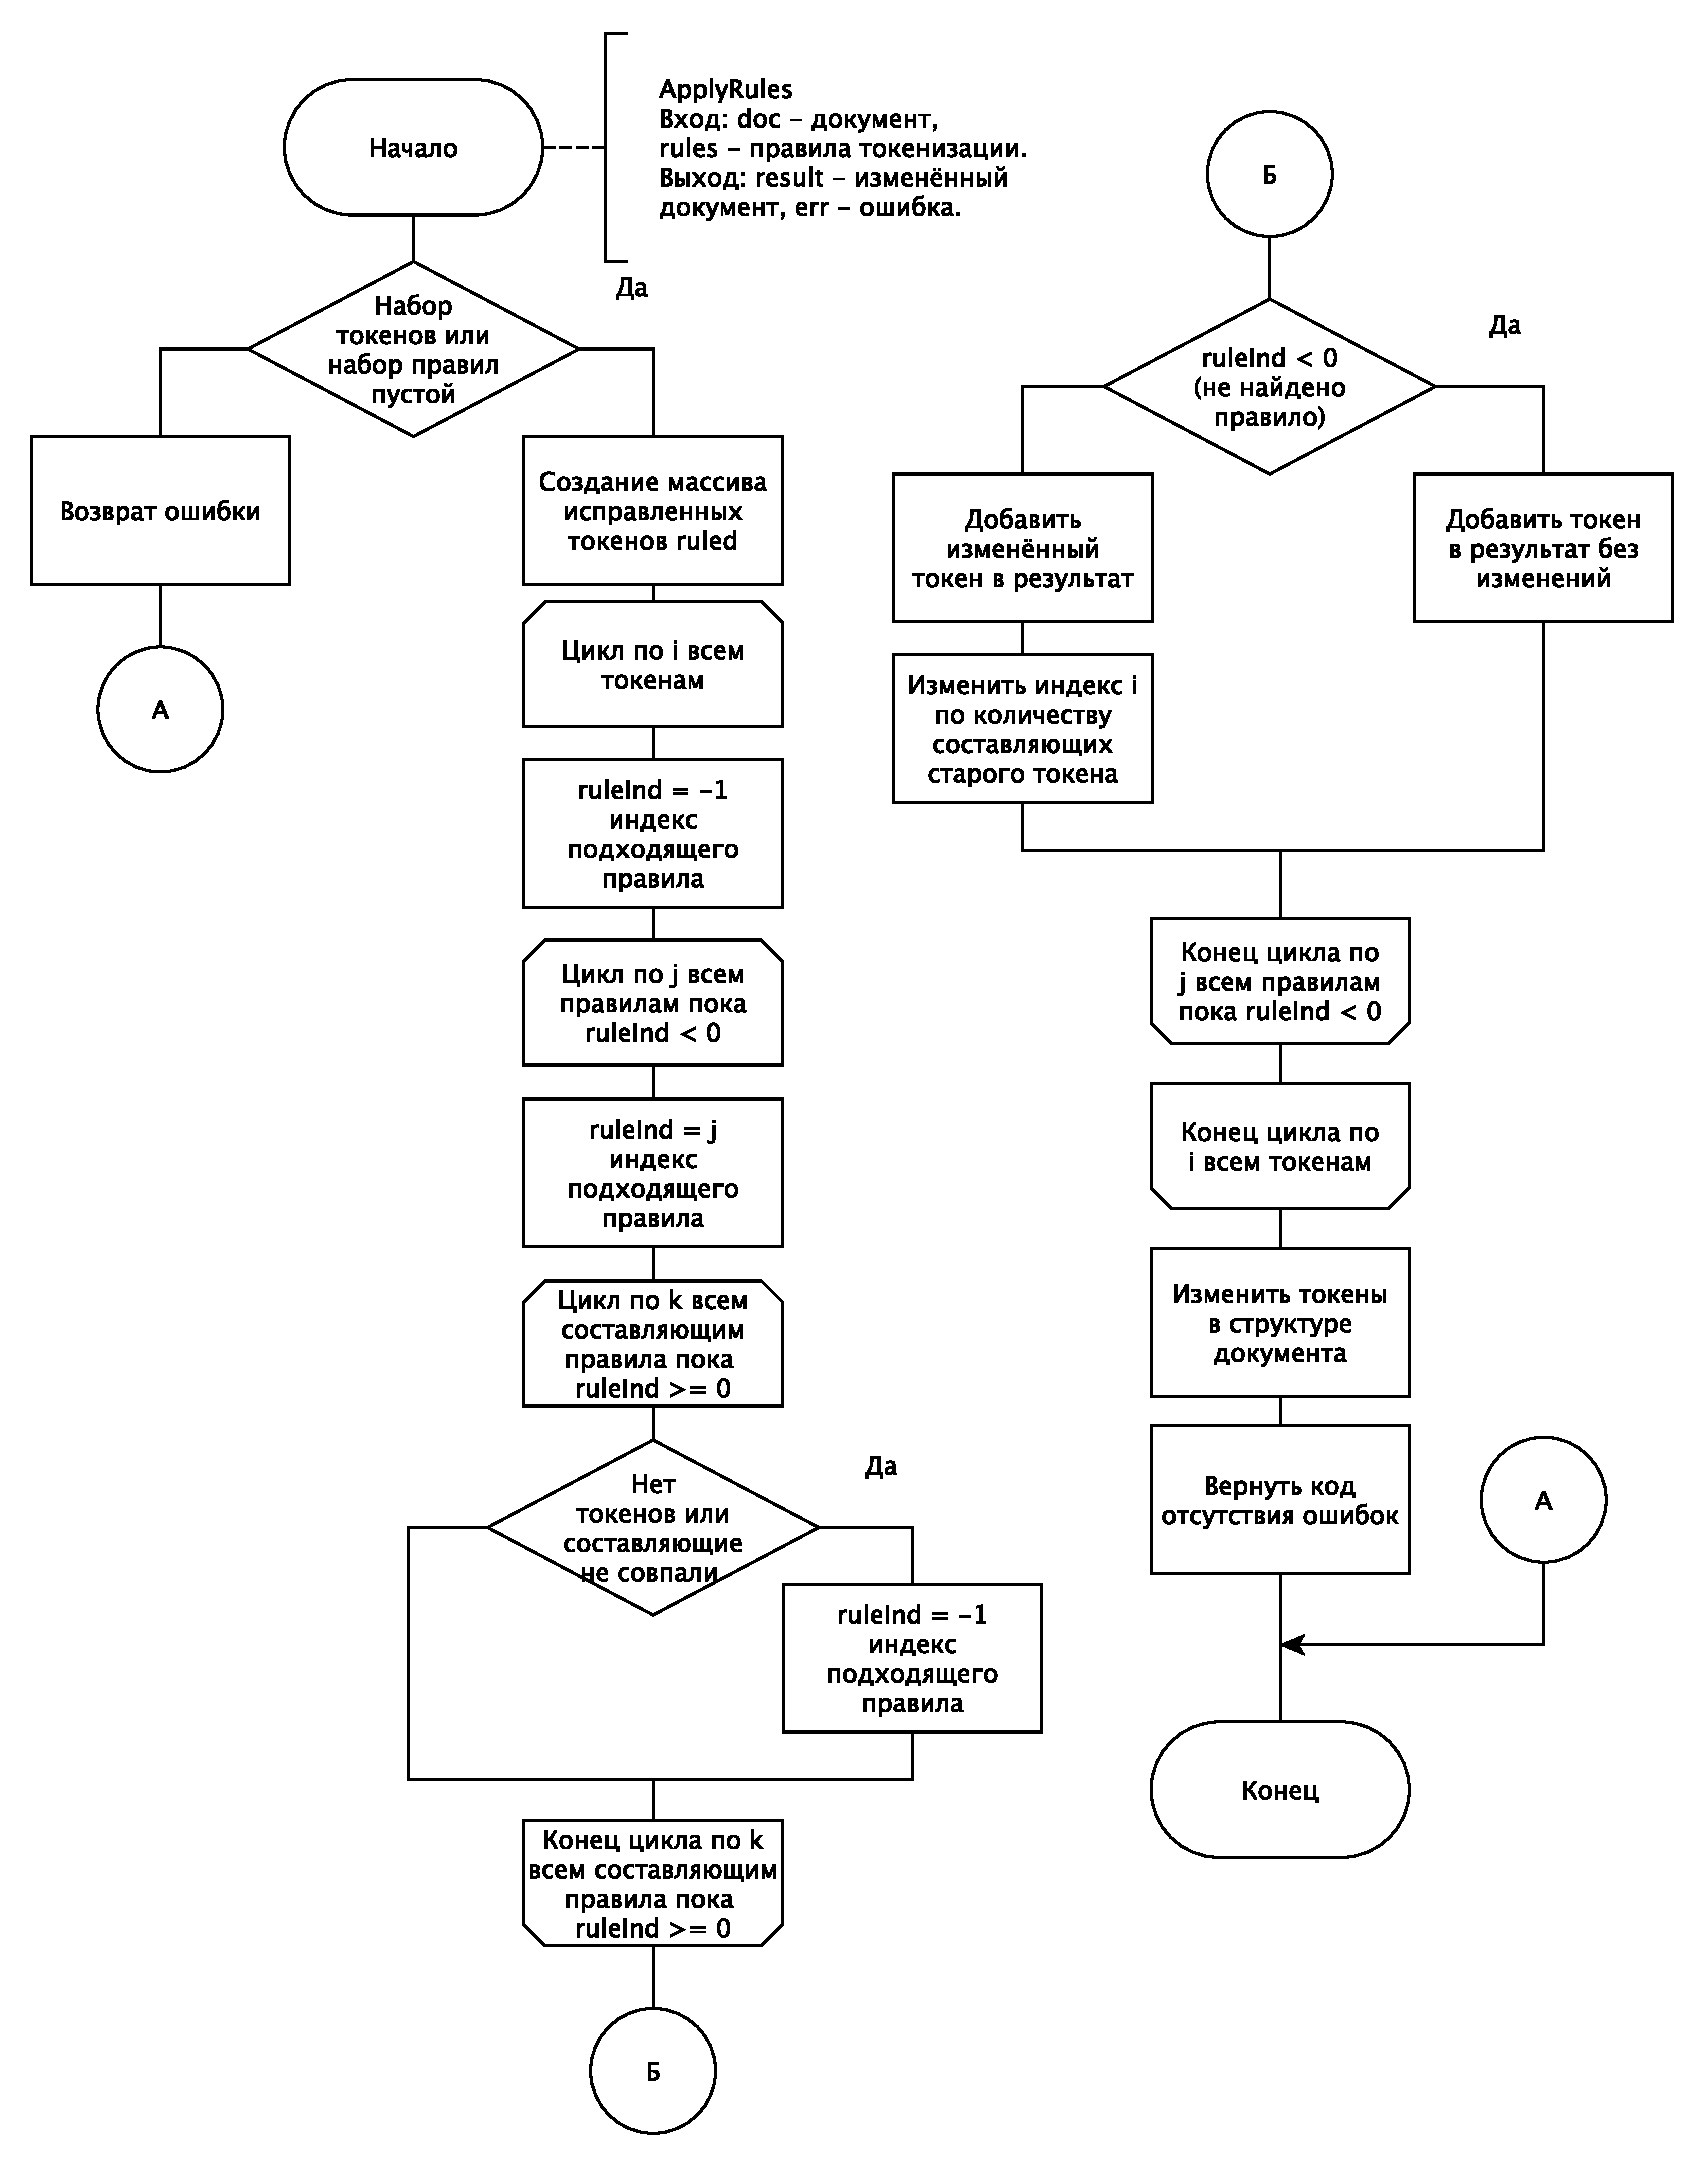
\includegraphics[width=0.8\linewidth]{rule.pdf}
    \caption{Схема реализации алгоритма применения правил к токенам текста}
    \label{img:rule}
\end{figure}

\section{Разработка алгоритма сортировки токенов по алфавиту}
Разработка алгоритма сортировки токенов по алфавиту исключается из рассмотрения в связи с наличием готовых решений, не требующих разработки \cite{web_item14}.

\newpage